%% replace 'papertag' with short distinct tag
%% - helps with distinction for inclusion in other documents
%% - always

%% procedure for figures:
%% adding directory figures/localized/
%% before figures in includegraphics
%% commands forces search and localize

\section{Introduction}
\label{sec:papertag.introduction}

\begin{figure}[tp!]
  \centering	
    
\includegraphics[width=0.5\columnwidth]{figures/localized/Garak.jpg}  
  \caption{
    Garak, tailor and retired (?) spymaster.
  }
  \label{fig:papertag.}
\end{figure}

\section{Description of data sets}
\label{sec:papertag.data}

Transcripts of all episodes of \textit{Star Trek: The Original Series}, \textit{The Next Generation} and \textit{Deep Space Nine}, as obtained from \href{http://chakoteya.net/StarTrek/index.html}{chakoteya.net} in February 2023. These are the first three live-action series of the Star Trek franchise, originally released from 1966-1969, 1987-1994 and 1993-1999, respectively.

\section{Model}
\label{sec:papertag.model}

\section{Results}
\label{sec:papertag.results}

\todo{Explain what we found}

\begin{figure}
    \centering
    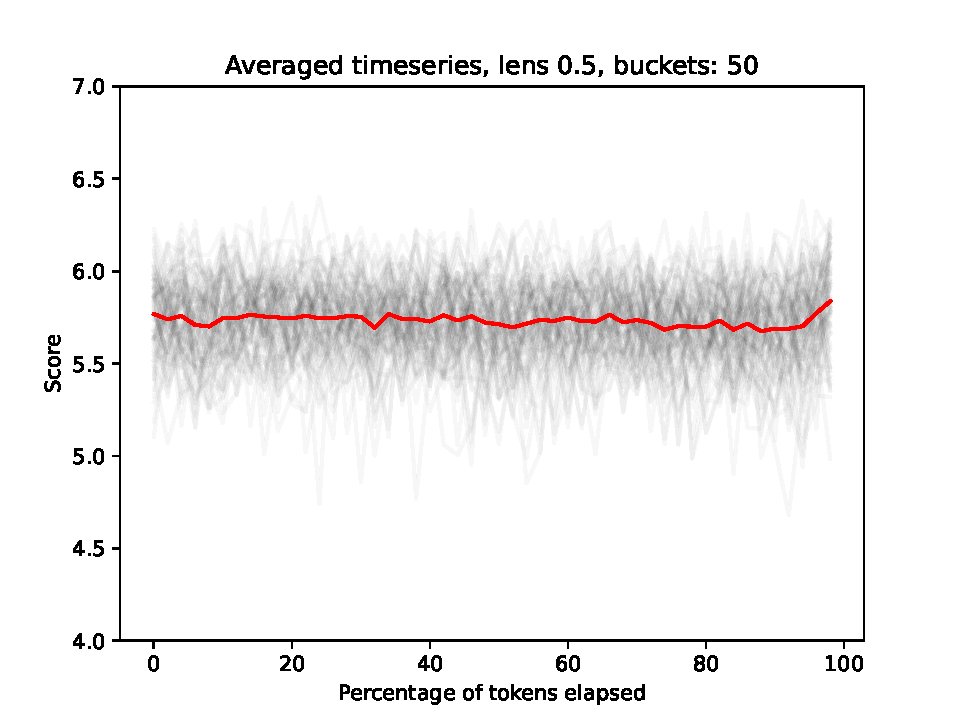
\includegraphics[width=\columnwidth]{figures/localized/average_episode_tos.pdf}
    \caption{Happiness timeseries of the average episode of Star Trek: The Original Series. Episodes are scaled to the length of the shortest episode. All episodes plotted in black, the red line is the average.}
    \label{fig:average_episode_tos}
\end{figure}

\begin{figure}
    \centering
    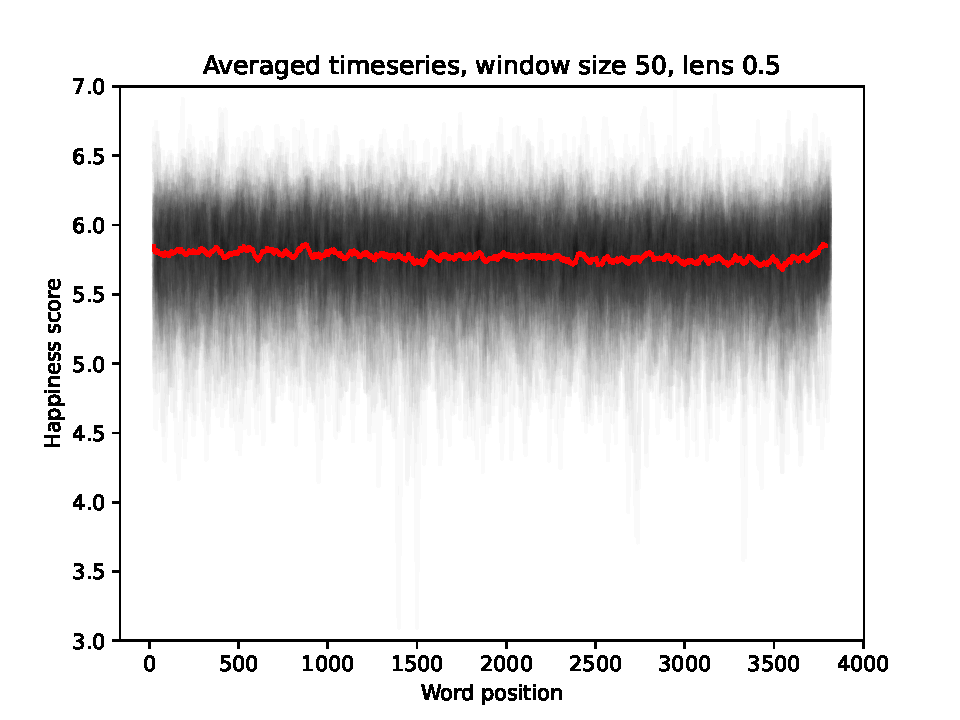
\includegraphics[width=\columnwidth]{figures/localized/average_episode_tng.pdf}
    \caption{Happiness timeseries of the average episode of Star Trek: The Next Generation. Episodes are scaled to the length of the shortest episode. All episodes plotted in black, the red line is the average.}
    \label{fig:average_episode_tng}
\end{figure}

\begin{figure}
    \centering
    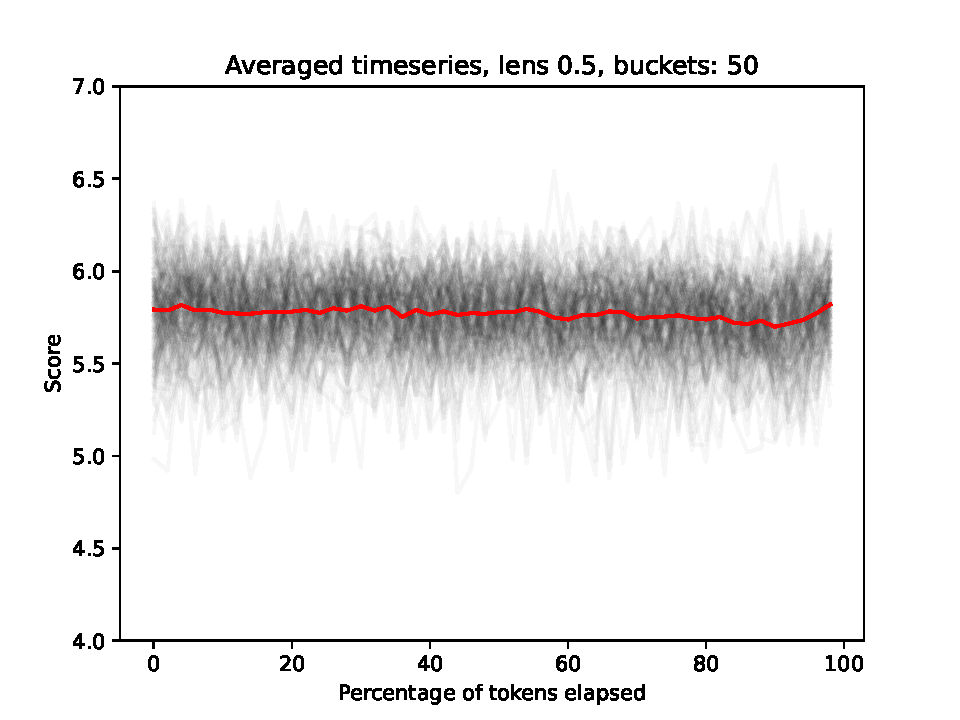
\includegraphics[width=\columnwidth]{figures/localized/average_episode_ds9.pdf}
    \caption{Happiness timeseries of the average episode of Star Trek: Deep Space Nine. Episodes are scaled to the length of the shortest episode. All episodes plotted in black, the red line is the average.}
    \label{fig:average_episode_ds9}
\end{figure}

Visible in \ref{fig:average_episode_tos}, \ref{fig:average_episode_tng} and \ref{fig:average_episode_ds9}: The episodes usually have a happy end in all three series. Average happiness is comparable overall.

\section{Concluding remarks}
\label{sec:papertag.concludingremarks}

\todo{Bring it home.}

\section{Methods}
\label{sec:papertag.methods}

\todo{Add methods.}
